\ifdefined\AUDITBLINDED
\documentclass[preprint,12pt,doubleblind]{elsarticle}
\else
\documentclass[preprint,12pt]{elsarticle}
\fi

\input{glyphtounicode}
\pdfgentounicode=1
\usepackage[T1]{fontenc}
\usepackage{lmodern}
\usepackage{amsmath}
\usepackage{amssymb}
\usepackage{array}
\usepackage{tabularx}
\usepackage{booktabs}
\usepackage{graphicx}
\usepackage{placeins}
\usepackage{tikz}
\usepackage{xurl}
\usepackage[protrusion=true,expansion=false]{microtype}
\usetikzlibrary{arrows.meta,positioning,calc,fit,backgrounds}
\setlength{\emergencystretch}{2em}
\newcommand{\best}[1]{\textbf{#1}}
\newcommand{\COtwo}{CO\textsubscript{2}}

\journal{Biosystems Engineering}

\begin{document}

\begin{frontmatter}

\title{Sensor faults and actuator commands in a low-cost closed hydroponic system: a retrospective audit}

\ifdefined\AUDITBLINDED
\else
\author[du]{MD. Sameer Iqbal Chowdhury}
\author[du]{Mikdam-Al-Maad Ronoue}
\author[kuas]{Md Asaduzzaman}
\author[du]{Lafifa Jamal\corref{cor1}}
\cortext[cor1]{Corresponding author.}
\affiliation[du]{organization={Department of Robotics and Mechatronics Engineering, University of Dhaka}, postcode={Dhaka-1000}, country={Bangladesh}}
\affiliation[kuas]{organization={Department of Agriculture and Food Technology, Kyoto University of Advanced Sciences}, country={Japan}}
\fi

\begin{abstract}
We audit how sensor faults can propagate into actuator commands in a low-cost Internet of Things hydroponic controller. A 30-day closed nutrient film technique lettuce deployment produced 121,244 logged samples, including impossible pH values, prolonged full-scale readings, and gaps covering 23\% of the period. Replay enforces the deployed setpoints, cooldown, and executable actuator directions. Under naive control, flagged readings supplied 19.1\% of pH dosing commands and 10.2\% of \COtwo{} injection commands. A physical-range check with 32~s persistence reduced these fractions to zero and 2.0\%. Flags distinguish out-of-range values, bound readings, and heuristic spikes; they are not independent fault diagnoses. Only 3\% of valid air-temperature readings and 10\% of valid water-temperature readings were in band, indicating poor regulation with an unresolved cause. LiveGate, a forecast-consistency and sensor-liveness gate, did not outperform simple baselines overall under a frozen retrospective protocol. A post-hoc comparison with run-length and bound-rejection gates exposed substantial availability costs. Learned liveness reduced commands using injected stuck readings by 79\%, but useful-command coverage in those trials fell from 98\% to 27\%. Commands were reconstructed, not observed; actual dosing, prevented damage, and crop benefits remain unmeasured.
\end{abstract}

\begin{keyword}
hydroponics \sep sensor faults \sep actuation \sep retrospective audit
\end{keyword}

\end{frontmatter}

\section{Introduction}
Closed hydroponic systems recirculate a nutrient solution whose pH, electrical conductivity (EC), and temperature must be held within narrow ranges, while the surrounding air temperature, humidity, and carbon dioxide (\COtwo) concentration shape growth in enclosed production \cite{niu2022hydroponics,asaduzzaman2022nutrients}. Automated controllers built from low-cost sensors, microcontrollers, and single-board computers now regulate these quantities with dosing pumps, valves, chillers, and coolers \cite{domingues2012automated,tatas2022reliable}. In such controllers a sensor reading is not only a data point: it can trigger a physical action. One spurious high pH reading can authorize acid dosing into the whole recirculating volume, and the correction may require dilution, counter-dosing, and another mixing interval.

System studies of IoT hydroponics describe architectures, dashboards, and crop outcomes, while sensor-fault studies characterize faults and their detection \cite{ni2009faulttypes,sharma2010sensorfaults,teh2020sensorquality,zou2023agriiotfaults}. SensorTalk already connects agricultural fault diagnosis to relationships between sensors and actuators \cite{lin2019sensortalk}. The narrower question here is how flagged readings change executable command counts under a specified controller, and how much useful authorization is lost when readings are rejected. This requires accounting for actuator direction, persistence, cooldown, and the age of held readings together.

This paper addresses that gap with data from a deployed closed NFT lettuce system. Its contributions are:
\begin{enumerate}
\item a descriptive inventory of invalid, spiking, repeated, and missing readings in a 30-day hydroponic deployment;
\item an executable-command replay that attributes authorizations to their source readings and compares six gating rules;
\item a frozen retrospective comparison of LiveGate with 14 alternatives, reporting its negative overall result, followed by a separate comparison with simple run-length and physical-bound gates;
\item engineering implications for gating, instrumentation, and temperature regulation, with explicit limits on physical and agronomic inference.
\end{enumerate}

\section{Related work}
\subsection{IoT control of hydroponic systems}
Automated hydroponic control typically measures pH and EC in the nutrient tank and corrects them with acid, base, concentrate, or water dosing, often with a mixing delay between doses \cite{domingues2012automated}. IoT variants add networked logging and remote monitoring \cite{tatas2022reliable}. Reliability in these studies is usually discussed in terms of communication and uptime, and evaluation focuses on whether the controlled variables stay near their setpoints and on crop performance. How often the controller acts on readings that were wrong is rarely reported.

\subsection{Sensor faults and their detection}
Field sensor deployments exhibit outliers, spikes, stuck-at values, offsets, drift, and missing data \cite{ni2009faulttypes,sharma2010sensorfaults}, and data quality in IoT pipelines has been reviewed systematically \cite{teh2020sensorquality}. Reviews of agricultural IoT report similar fault classes and a growing set of model-based and learning-based detectors \cite{zou2023agriiotfaults}. Classical detectors include robust outlier filters \cite{hampel1974influence}, sequential change detectors such as CUSUM \cite{page1954continuous,basseville1993detection}, exponentially weighted moving averages \cite{roberts1959control}, state estimation with the Kalman filter \cite{kalman1960new}, and density-based novelty detection such as the local outlier factor (LOF) \cite{breunig2000lof}; model-based fault diagnosis is surveyed in \cite{isermann2005fault}. Most of these methods treat a reading that changes little as normal. A stuck or saturated sensor is therefore hard for them to detect, and persistence-based confirmation rules can even make such readings look more trustworthy.

\subsection{Conformal calibration}
Split conformal prediction converts a predictor into a set or threshold with a finite-sample coverage guarantee under exchangeability \cite{vovk2005algorithmic,angelopoulos2023gentle}. Here its quantile rule provides a nominal calibration parameter. We make no formal coverage guarantee for these dependent sensor time series; the nominal parameter is not a guaranteed clean-reading rejection rate, and performance is assessed empirically.

\section{System and deployment}
\subsection{Platform}
The platform is a closed NFT system for leaf lettuce consisting of a Growth Module and a Nutrient Solution Container Module (Fig.~\ref{fig:system}, Table~\ref{tab:components}). The Growth Module measures air temperature and humidity with a DHT22 sensor and \COtwo{} with an MH-Z19C non-dispersive infrared sensor whose range ends at 5000~ppm. \COtwo{} is raised by a normally closed solenoid valve on a \COtwo{} cylinder, air temperature is lowered by a thermoelectric cooler, and LED grow lights provide the photoperiod. The Nutrient Solution Container Module measures pH with an Atlas Scientific analog pH kit, EC with an Atlas Scientific Mini Conductivity K~1.0 kit, water temperature, and water level with a JSN-SR04T ultrasonic sensor. pH is corrected by acid or base dosing, EC by concentrate or distilled-water dosing, and water temperature by a refrigerative chiller. A pump circulates the solution continuously and an aerator runs throughout.

Sensors are read by an Arduino Nano, which applies median filtering; actuators are driven by an Arduino Mega; a Raspberry Pi~4 Model~B runs the controller and uploads readings to a ThingSpeak channel at about 16~s intervals. Actuator commands and relay states were not logged.

\begin{figure}[!htbp]
\centering
\resizebox{\linewidth}{!}{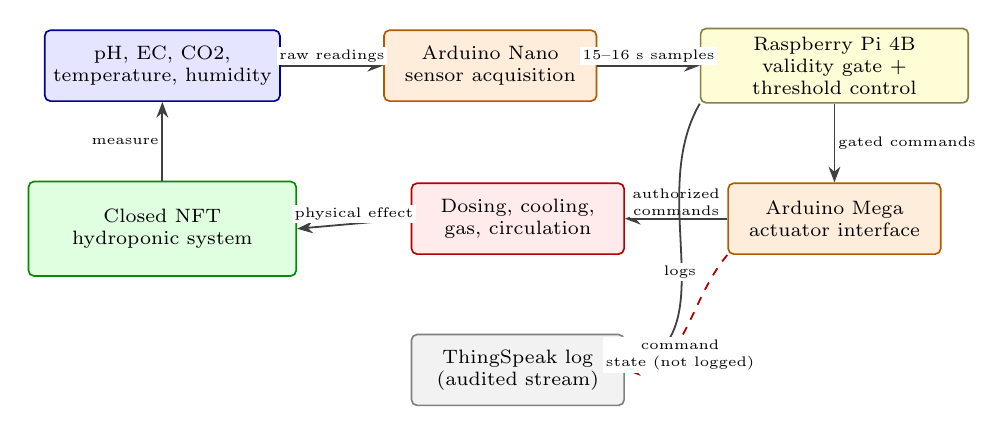
\begin{tikzpicture}[node distance=10mm and 13mm]
\tikzset{
  block/.style={rectangle, rounded corners=2pt, draw=black!70, line width=0.6pt,
    minimum width=27mm, minimum height=9mm, align=center, font=\scriptsize, inner sep=3pt},
  process/.style={block, fill=green!12, draw=green!55!black, minimum width=34mm, minimum height=12mm},
  sense/.style={block, fill=blue!10, draw=blue!60!black},
  compute/.style={block, fill=orange!14, draw=orange!70!black},
  guard/.style={block, fill=yellow!16, draw=yellow!45!black, minimum width=34mm},
  act/.style={block, fill=red!8, draw=red!70!black},
  data/.style={block, fill=gray!10, draw=black!50},
  flow/.style={-{Stealth[length=2mm,width=1.5mm]}, line width=0.65pt, draw=black!75},
  stop/.style={-{Stealth[length=2mm,width=1.5mm]}, dashed, line width=0.65pt, draw=red!70!black},
  lab/.style={font=\tiny, align=center, fill=white, inner sep=1pt}
}

\node[process] (hydro) {Closed NFT\\hydroponic system};
\node[sense, above=of hydro] (sensors) {pH, EC, CO2,\\temperature, humidity};
\node[compute, right=of sensors] (nano) {Arduino Nano\\sensor acquisition};
\node[guard, right=of nano] (pi) {Raspberry Pi 4B\\validity gate +\\ threshold control};
\node[compute, below=of pi] (mega) {Arduino Mega\\actuator interface};
\node[act, left=of mega] (actuators) {Dosing, cooling,\\gas, circulation};
\node[data, below=of actuators] (log) {ThingSpeak log\\(audited stream)};

\draw[flow] (hydro) -- node[lab, left] {measure} (sensors);
\draw[flow] (sensors) -- node[lab, above] {raw readings} (nano);
\draw[flow] (nano) -- node[lab, above] {15--16 s samples} (pi);
\draw[flow] (pi) -- node[lab, right] {gated commands} (mega);
\draw[flow] (mega) -- node[lab, above] {authorized\\commands} (actuators);
\draw[flow] (actuators.west) -- node[lab, above] {physical effect} (hydro.east);
\draw[flow] (pi.south west) to[out=-120,in=20] node[lab, pos=0.58, above] {logs} (log.east);
\draw[stop] (mega.south west) to[out=-130,in=0] node[lab, pos=0.55, below] {command\\state (not logged)} (log.east);
\end{tikzpicture}
}
\par\medskip
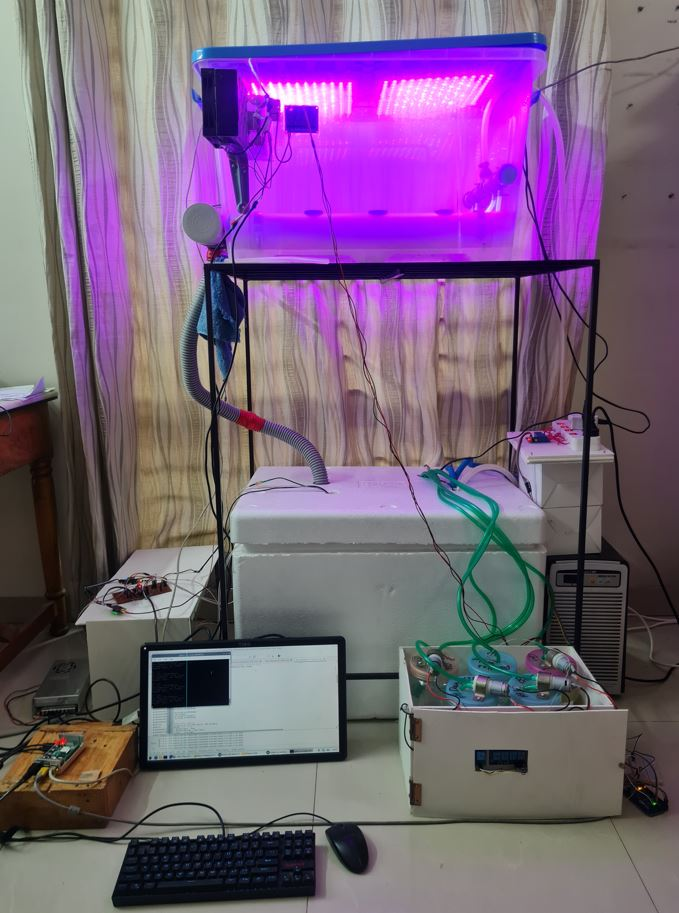
\includegraphics[height=4.3cm]{figure/fullsystemactual.JPG}
\caption{Sensing-to-actuation path (top) and the deployed NFT system (bottom). Sensor readings were logged; command and relay states were not recorded.}
\label{fig:system}
\end{figure}

\begin{table}[!htbp]
\centering
\caption{Controlled quantities, deployed setpoint bands, and the directions the installed actuators can execute. Humidity and water level were monitored but not actuated.}
\label{tab:components}
\small
\setlength{\tabcolsep}{4pt}
\begin{tabularx}{\linewidth}{@{}l l X l@{}}
\toprule
Quantity & Setpoint band & Actuator & Executable direction \\
\midrule
pH & 5.8--6.5 & Acid / base dosing & Both \\
EC & 1000--1500~\textmu S\,cm$^{-1}$ & Water / concentrate dosing & Both \\
\COtwo & 1900--2100~ppm & Solenoid valve on cylinder & Raise only \\
Water temperature & 18--22~\textdegree C & Refrigerative chiller & Lower only \\
Air temperature & 20--26~\textdegree C & Thermoelectric cooler & Lower only \\
\bottomrule
\end{tabularx}
\end{table}

\subsection{Control law and the deployed gating rule}
The controller issues a correction when a reading leaves its setpoint band, then locks the corresponding dosing subsystem for 10~min to allow mixing. In the first growing season the controller acted on logged readings without further gating. In the second season, which produced the log analysed here, it used an error-resilience rule: a reading was accepted only if it differed from the last trusted value by at most $(1+\beta)\xi$, where $\xi$ is the mean absolute change between successive readings; after 50 consecutive rejections the trusted value was reset to the current reading; and a correction required $\psi$ consecutive accepted out-of-band readings, where $\psi$ is the mean length of runs of small successive changes. The published multipliers $\beta$ were 0.0002 (EC), 0.0005 (pH), 0.0022 (air temperature), 0.0009 (water temperature), and 0.0010 (\COtwo).

\subsection{Deployment}
The analysed deployment ran from 27 February to 28 March 2024 in Dhaka, Bangladesh, with ambient temperatures of about 25--36~\textdegree C, which is off-season for lettuce. Seven seedlings per treatment were grown in the NFT system, in pots with soil and compost, and in a manually managed deep water culture (DWC) system.

\section{Methods}
\subsection{Data}
The log contains 121,244 rows with a median interval of 16~s. The analysis uses the five actuated quantities, plus humidity for the fault inventory. Water level is excluded because its raw values were never calibrated to a physical level. Timestamps are split chronologically into development (first 40\%), validation (next 30\%), and evaluation (last 30\%) blocks.

\subsection{Fault inventory}
For each channel we count readings outside the physical range ($0$--$14$ for pH, $0$--$5000$~\textmu S\,cm$^{-1}$ for EC, $250$--$5000$~ppm for \COtwo, $-10$--$60$~\textdegree C for air and $0$--$50$~\textdegree C for water temperature, $0$--$100$\% for humidity); isolated spikes, defined as in-range readings whose deviation from a centred 9-sample median exceeds eight robust standard deviations; flat-line runs of identical readings lasting at least 1~h without a logging gap; the fraction of readings at the channel's in-range maximum; and logging gaps longer than 120~s. These are descriptive definitions, not ground-truth labels.

\subsection{Fault-to-actuation audit}
The audit replays the deployed setpoint bands and a 10-min cooldown on the unmodified log under six gating arms: (i) a naive threshold on every logged reading, as in the first season; (ii) a physical-range check; (iii) a range check with 32~s persistence before acting; (iv) the deployed error-resilience rule, reconstructed from its description with the published $\beta$ values and with $\xi$ and $\psi$ re-estimated on the development block because the first-season data used originally are unavailable; (v) arm (iii) plus the LiveGate liveness test (Section~\ref{sec:livegate}); and (vi) arm (iii) plus rejection of readings exactly at a declared physical bound. The last accepted value may be held for at most 64~s; a logging gap longer than 120~s invalidates it. Directions unavailable to the installed actuator are suppressed before persistence and cooldown are evaluated. An unavailable direction therefore cannot delay a later executable command.

Each command is attributed to the reading supplying its held estimate. We report three disjoint flag categories: out-of-range values, readings exactly at a declared bound, and in-range isolated spikes not already at a bound. A bound reading may represent a true excursion beyond the sensor's range, and a spike may be a legitimate transient; neither is an independently confirmed sensor fault. The replay uses a fixed historical background: its commands do not change subsequent readings. It therefore measures authorization differences, not actual dosing, prevented damage, or crop effects. Band occupancy is the fraction of logged readings within range and away from declared bounds that fall inside the setpoint band; it is not a duration-weighted estimate for missing periods.

\subsection{Controlled benchmark}
Because the log has no actuator records or reference instruments, faults that cannot be identified from the log alone are studied with controlled injection into real backgrounds. Eight non-overlapping, gap-free 240-sample windows are drawn from each of the validation and evaluation blocks. In each window, one of 12 scenarios is applied to one channel after a 60-sample warm-up: clean; positive or negative spikes, 30-sample biases, and 30-sample drifts; a 30-sample stuck value; 30 samples pinned at the declared physical maximum (saturation); a 30-sample dropout; and positive or negative legitimate level shifts that also change the reference background. Magnitudes are 0.5 for pH, 100~\textmu S\,cm$^{-1}$ for EC, 2~\textdegree C for air and 1~\textdegree C for water temperature, and 500~ppm for \COtwo.

Every method produces an accepted/rejected decision for each reading. A common downstream controller holds the last accepted value for up to a maximum age (64 or 320~s), requires out-of-band persistence (0, 32, or 96~s), and applies the 10-min cooldown. Reference opportunities are defined from the uncorrupted background with fixed 32~s persistence and the same cooldown; an authorization matches an opportunity if it occurs in the same out-of-band episode and direction within 180~s. Coverage is the fraction of reference opportunities matched; undesirable authorizations are commands issued when the background is in band or in the opposite direction. The benchmark retains the frozen protocol's idealized two-direction controller for every channel; these counts are distinct from the executable-command audit.

Two secondary metrics distinguish authorizations occurring during injected-fault samples from authorizations whose last accepted source reading was fault-labelled. The former is the original protocol's temporal-coincidence metric; it does not establish use of a corrupted reading. The latter follows the held estimate's provenance, including commands after a fault ends. Neither metric alone establishes an undesirable direction relative to the background.

Each method's detector setting, persistence, and maximum age are selected on validation windows at three coverage targets (0.5, 0.8, 0.95): among settings meeting the target, the one with the fewest undesirable authorizations per trial is locked, and evaluation windows are then scored once. The 14 alternatives to full LiveGate comprise persistence only, Hampel, CUSUM, LOF, Kalman, EWMA, moving median, generalized likelihood ratio (GLR), three AASVR-R supervisor variants (measurement supervisor, hold-only, and without CUSUM), always-deny, and two LiveGate ablations. Kalman noise is scaled per channel from development data. Each split contains 480 channel--scenario trials derived from eight source windows; the evaluation windows span seven source days, not 480 independent deployments. Paired 95\% percentile intervals resample those days jointly across sensors and scenarios with 1000 bootstrap replicates \cite{efron1979bootstrap}. Seven clusters provide limited information about between-day variability. Component intervals are descriptive, without multiplicity adjustment; settings remain fixed during resampling.

\subsection{LiveGate}
\label{sec:livegate}
LiveGate accepts a reading $y_t$ for actuation only if it is consistent with a learned forecast and the sensor appears alive.

\paragraph{Consistency} Let $\ell_t$ be the mean of the last $K=5$ accepted readings and $\tau_t$ the difference between the newest and oldest of them. The forecast is
\begin{equation}
\hat{y}_t = \ell_t + \mathbf{w}^\top \boldsymbol{\phi}_t + b,\qquad
\boldsymbol{\phi}_t = \big[\tau_t,\ \sin(2\pi h_t/24),\ \cos(2\pi h_t/24),\ \mathbf{z}_t\big],
\end{equation}
where $h_t$ is the hour of day and $\mathbf{z}_t$ contains the other four actuated channels, winsorized at their development 1st and 99th percentiles and centred at their medians. The weights are fitted by Huber regression \cite{huber1964robust} of $y_t-\ell_t$ on the first 75\% of the development block, using only in-range, non-spike readings. The score is $s_t=|y_t-\hat{y}_t|/\sigma$, where $\sigma$ is 1.4826 times the median absolute training residual. The threshold is the split-conformal quantile
\begin{equation}
q_\varepsilon = s_{(\lceil (n+1)(1-\varepsilon) \rceil)}
\end{equation}
of the $n$ clean scores in the last 25\% of the development block.

\paragraph{Liveness} Let $r_t$ be the length of the current run of identical readings. From the $N$ runs of filtered readings in the first 75\% of development, excluding readings at a declared physical bound, the smoothed survival function is $S(r)=(|\{\text{runs}\ge r\}|+1)/(N+1)$. The sensor is considered alive while $S(r_t)\ge\varepsilon$. The frozen implementation counts training runs after filtering and does not reset its liveness counter at logging gaps. The controlled comparison uses gap-free windows; whole-log liveness results remain subject to this gap-handling limitation.

\paragraph{Decision} A reading is accepted if it is within the physical range, the sensor is alive, and $s_t\le q_\varepsilon$. A live but surprising reading starts a candidate level, and the trusted state re-anchors after
\begin{equation}
m(s_t) = \mathrm{clip}\big(1+\lceil \log_2(s_t/q_\varepsilon)\rceil,\ 2,\ 8\big)
\end{equation}
mutually consistent readings, so larger surprises require more confirmation. The single parameter $\varepsilon\in\{0.002,0.01,0.05\}$ sets both the consistency and liveness thresholds and takes the place of the baselines' threshold multipliers.

\paragraph{Protocol} The method, the benchmark, and the decision rules were committed to the project repository before LiveGate was run on the measured log. LiveGate would be called best at a coverage target only if it had the lowest evaluation undesirable rate among methods feasible at that target, with coverage within 0.02 of the best feasible method; and best overall only if this held at every target where it was feasible. One design change, anchoring the forecast on a 5-sample level rather than the last value, was made beforehand to fix cascading rejections found in synthetic unit tests. The data had been analysed in earlier studies, so the evaluation is retrospective rather than on untouched data.

\section{Results}
\subsection{Faults in the deployment log}
Flagged readings were frequent and channel-specific (Table~\ref{tab:inventory}, Fig.~\ref{fig:heatmap}). pH produced 464 physically impossible readings, up to 67,101, consistent with corrupted analog or serial transfers, although the fault location cannot be diagnosed from the log. \COtwo{} produced 819 out-of-range readings, up to 200,850~ppm, and 961 isolated spike flags; 2.3\% of its samples were exactly at the 5000~ppm full scale, including one 8.5~h episode. Humidity read 99.9\% for 99.97\% of samples. Saturation, sustained near-condensation conditions, and a stuck or corrupted channel cannot be distinguished without independent measurements. EC and both temperature channels had fewer flags; this does not establish their calibration accuracy. All channels shared 194 logging gaps longer than 120~s, the longest lasting 9.0~h, together covering 23\% of the deployment.

\begin{table}[!htbp]
\centering
\caption{Fault inventory of the 30-day deployment log (121,244 readings per channel). Spikes are in-range readings more than eight robust standard deviations from a centred 9-sample median.}
\label{tab:inventory}
\small
\setlength{\tabcolsep}{4pt}
\begin{tabular}{lrrrrr}
\toprule
Channel & \shortstack{Out of\\range} & \shortstack{Maximum\\out-of-range} & Spikes & \shortstack{Flat-lines\\$\ge$1~h} & \shortstack{Longest\\(h)} \\
\midrule
pH & 464 & 67,101 & 76 & 0 & -- \\
EC & 0 & -- & 14 & 0 & -- \\
\COtwo & 819 & 200,850 & 961 & 3 & 8.5 \\
Air temperature & 1 & 99.9 & 17 & 1 & 1.4 \\
Water temperature & 0 & -- & 39 & 7 & 1.5 \\
Humidity & 0 & -- & 10 & 79 & 35.2 \\
\bottomrule
\end{tabular}
\end{table}

\begin{figure}[!htbp]
\centering
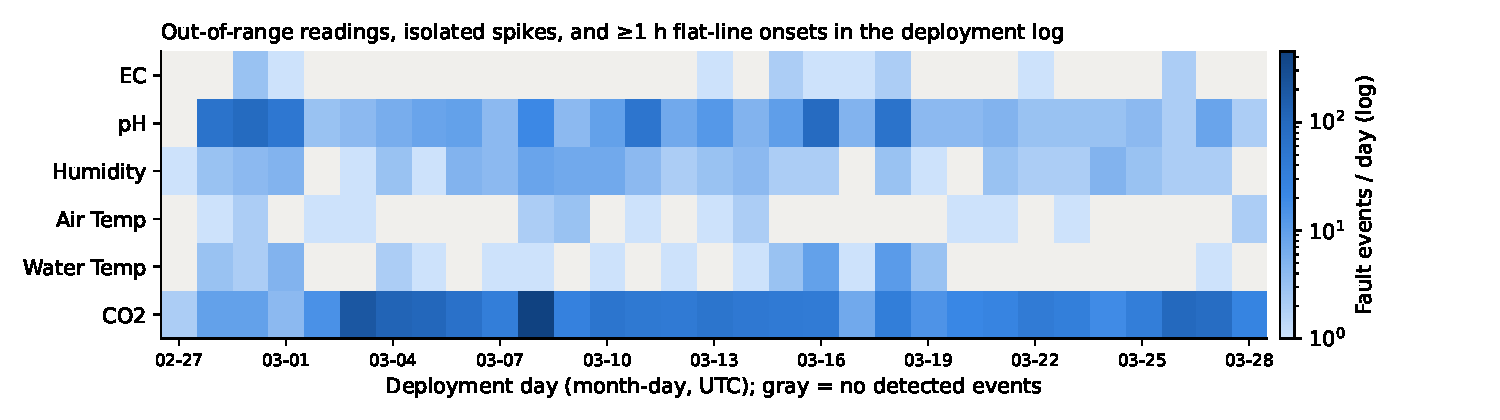
\includegraphics[width=\linewidth]{figure/audit/real_fault_heatmap.pdf}
\caption{Daily descriptive flags: out-of-range readings, isolated spikes, and onsets of flat-lines lasting at least 1~h. These flags are not independent diagnoses of sensor faults.}
\label{fig:heatmap}
\end{figure}

The long \COtwo{} episode was preceded by a steady rise from about 2000 to 5000~ppm over 2~h (Fig.~\ref{fig:co2}). The true concentration may have exceeded the sensor range, for example through a valve that failed open, but reference and valve-state measurements are absent. If the sensor was functioning and clipped at full scale, the reading gives a lower bound; if it was stuck, even that interpretation is unavailable. The replayed liveness test rejected the pinned readings within four samples.

\begin{figure}[!htbp]
\centering
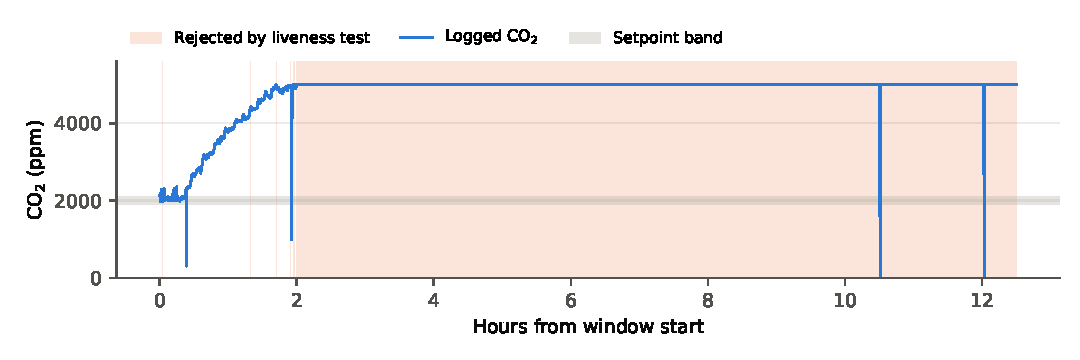
\includegraphics[width=\linewidth]{figure/audit/co2_saturation_trace.pdf}
\caption{Longest \COtwo{} full-scale episode, with readings rejected by the replayed liveness test ($\varepsilon=0.05$) shaded. Downward excursions are spike candidates; their physical cause is unverified.}
\label{fig:co2}
\end{figure}

\subsection{Observed regulation}
Among valid logged readings, 88\% of pH, 84\% of EC, and 47\% of \COtwo{} readings were in band (Fig.~\ref{fig:band}). Only 3\% of valid air-temperature readings were within 20--26~\textdegree C (median 28.6~\textdegree C), and 10\% of valid water-temperature readings were within 18--22~\textdegree C (median 24.8~\textdegree C). These sample proportions do not describe the unobserved 23\% of the deployment. The traces indicate poor temperature regulation, consistent with insufficient cooling capacity under hot-season conditions. Actuator failure, control problems, and calibration error remain possible; without command, relay, reference, and capacity measurements, the log cannot identify the cause or actual cooling duty.

\begin{figure}[!htbp]
\centering
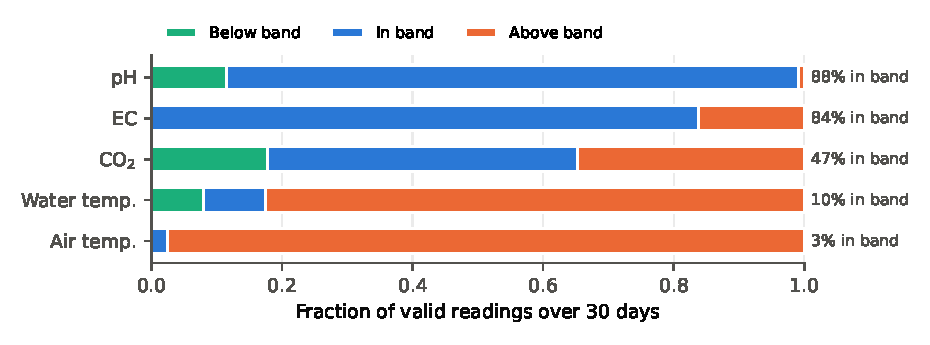
\includegraphics[width=0.85\linewidth]{figure/audit/time_in_band.pdf}
\caption{Fraction of valid readings below, within, and above each setpoint band over the deployment.}
\label{fig:band}
\end{figure}

\subsection{Fault-to-actuation audit}
A naive controller replay issued 655 pH dosing commands, of which 125 (19.1\%) used flagged readings, and 2149 \COtwo{} injection commands, of which 219 (10.2\%) used flagged readings (Table~\ref{tab:audit}, Fig.~\ref{fig:audit}). The pH flags comprise 89 out-of-range values, 25 bound readings, and 11 heuristic spikes; the \COtwo{} flags comprise 74 out-of-range values and 145 spikes. A range check left 40 flagged pH commands: 28 bound readings and 12 spikes. Adding 32~s persistence removed all flagged pH and EC commands and reduced flagged \COtwo{} injections to 9 of 456 (2.0\%), all nine attributed to heuristic spikes. Liveness and bound rejection produced the same executable \COtwo{} counts because high full-scale readings do not request injection in a raise-only loop.

These results correct an implementation error in the initial audit, which discarded unavailable directions only after they had consumed cooldown. Enforcing directions before authorization changes naive \COtwo{} counts from 1010/68 total/flagged to 2149/219 and range-plus-persistence counts from 441/7 to 456/9. The two-sided pH and EC results are unchanged. The separate frozen controlled benchmark deliberately remains bidirectional.

The reconstructed deployed rule issued 43--72\% as many commands as the range-and-persistence arm, depending on the channel, because its repeatability requirement corresponded to about 2--7~min of confirmation. It nevertheless authorized 13 \COtwo{} injections using out-of-range readings: after 50 consecutive rejections its reset accepts the current sensor value.

\begin{table}[!htbp]
\centering
\caption{Executable replay commands and commands using flagged source readings (out-of-range, declared-bound, or heuristic-spike flags). Tot.: total commands; Flag.: commands using flagged readings. No actual command execution was logged.}
\label{tab:audit}
\small
\setlength{\tabcolsep}{4pt}
\begin{tabularx}{\linewidth}{@{}Xrrrrrr@{}}
\toprule
 & \multicolumn{2}{c}{pH dosing} & \multicolumn{2}{c}{EC dosing} & \multicolumn{2}{c}{\COtwo{} injection} \\
Gating arm & Tot. & Flag. & Tot. & Flag. & Tot. & Flag. \\
\midrule
Naive threshold & 655 & 125 & 535 & 6 & 2149 & 219 \\
Range check & 593 & 40 & 535 & 6 & 2105 & 148 \\
Range + persistence & 417 & \best{0} & 526 & \best{0} & 456 & 9 \\
Deployed (reconstructed) & 216 & \best{0} & 227 & \best{0} & 330 & 13 \\
Range + persistence + liveness & 417 & \best{0} & 526 & \best{0} & 456 & 9 \\
Range + persistence + bound & 417 & \best{0} & 526 & \best{0} & 456 & 9 \\
\bottomrule
\end{tabularx}
\end{table}

\begin{figure}[!htbp]
\centering
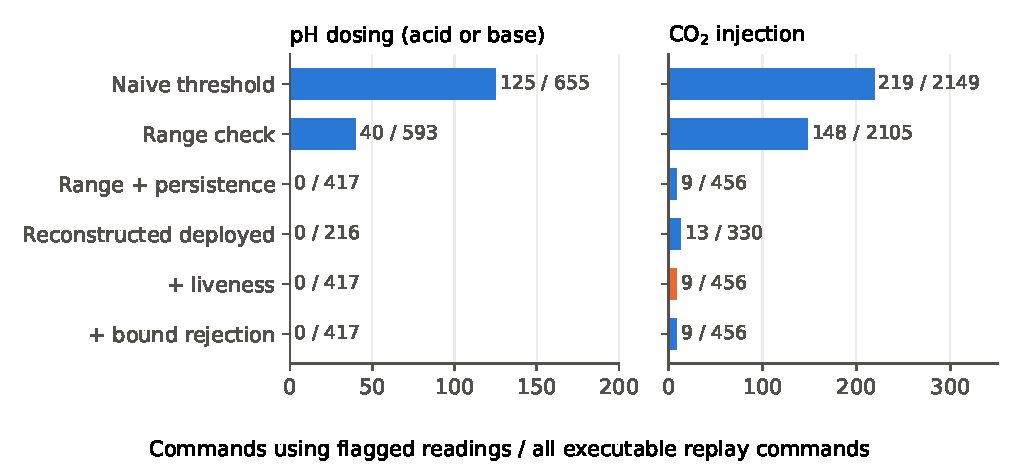
\includegraphics[width=\linewidth]{figure/audit/audit_fault_commands.pdf}
\caption{Executable replay commands using flagged readings, with counts relative to all executable commands under each arm. The flags do not establish physical harm.}
\label{fig:audit}
\end{figure}

The liveness test reduced replayed air-temperature cooling commands by 10\% (3215 to 2891) and water-temperature commands by 9\% (2698 to 2446). Coarsely quantized channels can repeat values during legitimate operation. These reductions are an authorization cost, not observed reductions in cooling or evidence of physical benefit.

\subsection{Controlled benchmark and the locked LiveGate result}
No method reached the 0.95 coverage target on validation. At the 0.5 and 0.8 targets, LiveGate did not meet the frozen criterion for best method (Table~\ref{tab:benchmark}). At 0.5, LOF had the fewest undesirable authorizations (0.075 per trial versus 0.135 for LiveGate; paired difference 95\% interval $-0.148$ to $-0.004$) but at much lower coverage (0.357). At 0.8, persistence only reached higher coverage (0.886) with fewer undesirable authorizations (0.117) than LiveGate (0.790 and 0.135). The liveness-only ablation had the lowest undesirable rate at 0.8 (0.104) but its evaluation coverage fell to 0.663. The AASVR-R measurement supervisor did not reach the 0.5 target. Figure~\ref{fig:operating} shows all validation operating points.

\begin{table}[!htbp]
\centering
\caption{Locked evaluation at the 180~s deadline. Settings were selected on validation; validation-infeasible methods are omitted. A dagger marks evaluation coverage below the corresponding target. Bold values are column extrema, not proof of an overall winner.}
\label{tab:benchmark}
\small
\begin{tabular}{llrr}
\toprule
Target & Method & Coverage & Undesirable / trial \\
\midrule
0.5 & LOF & $0.357^{\dagger}$ & \best{0.075} \\
 & LiveGate, liveness only & 0.560 & 0.081 \\
 & Kalman & 0.594 & 0.098 \\
 & GLR & 0.760 & 0.100 \\
 & Persistence only & 0.795 & 0.110 \\
 & CUSUM & 0.794 & 0.110 \\
 & Hampel / moving median & 0.795 & 0.121 \\
 & EWMA & \best{0.801} & 0.121 \\
 & LiveGate & 0.505 & 0.135 \\
 & LiveGate, forecast only & 0.704 & 0.163 \\
 & AASVR-R hold only & 0.721 & 0.233 \\
\midrule
0.8 & LiveGate, liveness only & $0.663^{\dagger}$ & \best{0.104} \\
 & Persistence only & 0.886 & 0.117 \\
 & CUSUM & 0.862 & 0.121 \\
 & LiveGate & $0.790^{\dagger}$ & 0.135 \\
 & Hampel / moving median & 0.848 & 0.150 \\
 & EWMA & 0.857 & 0.150 \\
 & LiveGate, forecast only & 0.837 & 0.150 \\
 & Kalman & \best{0.910} & 0.158 \\
 & GLR & 0.854 & 0.165 \\
\bottomrule
\end{tabular}
\end{table}

\begin{figure}[!htbp]
\centering
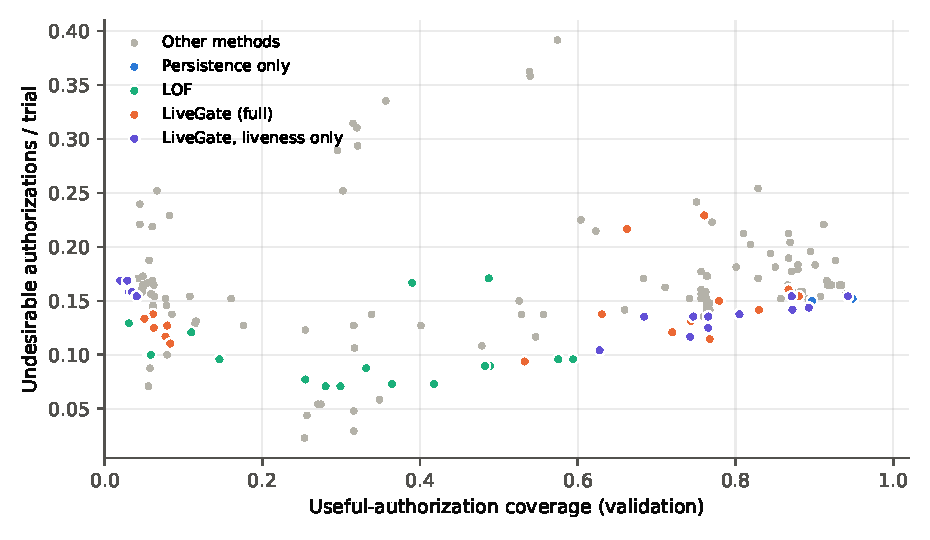
\includegraphics[width=\linewidth]{figure/audit/operating_points.pdf}
\caption{Validation operating points of all methods and settings. Points towards the lower right authorize more of the commands that are needed while issuing fewer that are not.}
\label{fig:operating}
\end{figure}

The forecast-only ablation rejected 3.2\% of uncorrupted readings at the 0.8 target, against none for persistence only, and had more undesirable authorizations (0.150 versus 0.117 per trial). Thus its extra rejection did not improve the aggregate authorization tradeoff in this benchmark. A fault and a legitimate change can produce the same local trace; additional context would have to be informative to distinguish them.

\subsection{Stuck and saturated sensors}
The original temporal-coincidence metric shows fewer authorizations during stuck and saturated intervals with liveness enabled (Fig.~\ref{fig:stuck}). At the 0.8 validation target, persistence only authorized during stuck samples 0.725 times per trial, compared with 0.225 for liveness only (69\% fewer) and 0.500 for full LiveGate. During saturation, the corresponding rates were 0.975, 0.675 (31\% fewer), and 0.650. Kalman reached 0.850; the other selected comparators matched persistence on this metric. These reductions do not by themselves show that fewer commands used corrupted source readings. They also accompany reduced overall coverage: 0.663 for liveness only versus 0.886 for persistence. The following analysis adds paired intervals, held-source attribution, and direct simple comparators.

\begin{figure}[!htbp]
\centering
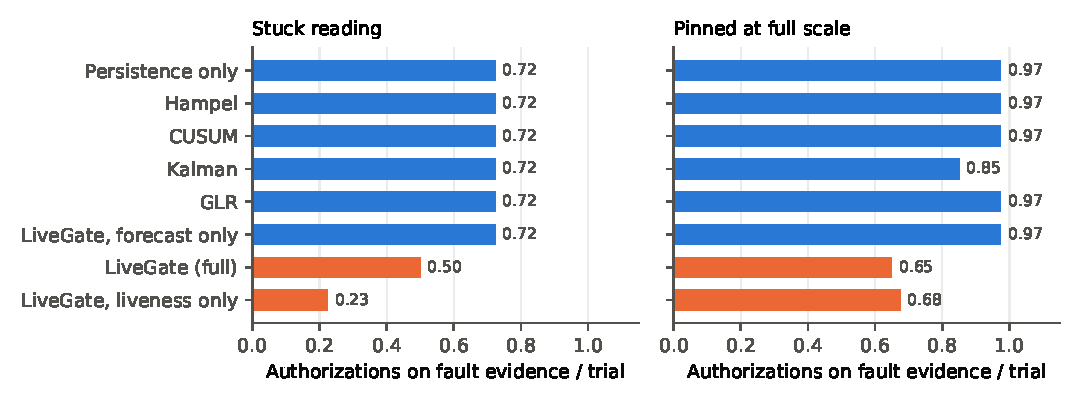
\includegraphics[width=\linewidth]{figure/audit/stuck_saturation.pdf}
\caption{Authorizations occurring during injected-fault samples, per trial (locked evaluation, 0.8 validation target). This temporal metric does not identify the source of a held estimate. Liveness arms are highlighted.}
\label{fig:stuck}
\end{figure}

\subsection{Exploratory post-hoc variant}
After the locked run, we tested one post-hoc change, labelled exploratory: flooring the forecast scale at each sensor's reading resolution, motivated by the near-zero scales fitted on the temperature channels. All benchmark settings and comparators were rerun, and every previously reported evaluation result reproduced exactly. The variant's selected settings, coverage, and undesirable rates were identical to those of locked LiveGate at both feasible targets. The change has no effect because the conformal threshold is calibrated on scores normalized by the same scale, so rescaling moves scores and threshold together. The forecast component's weakness is therefore not a scale artefact: across evaluation trials it rejected 3.2\% of clean readings at the 0.8 target, against none for persistence only, without reducing undesirable authorizations.

\subsection{Post-hoc direct-baseline comparison}

A separately labelled follow-up reran the original methods and added two direct comparators: a fixed repeat cap and rejection at either physical bound. The repeat cap accepts the first $R$ identical in-range readings, rejects subsequent repeats, and resets after a change, invalid reading, or logging gap. $R\in\{2,4,8,16,32,64\}$ is shared across channels; the six-value grid is larger than LiveGate's three-value grid. Both comparators use the original timing grid and validation-only selection. All original evaluation summary rows and selections reproduced, while the frozen artifacts remained unchanged. The follow-up is post-hoc because the data and original results had already been examined.

\begin{table}[!htbp]\centering\small\setlength{\tabcolsep}{4pt}

\caption{Post-hoc evaluation at the 0.8 validation coverage target. A dagger marks evaluation coverage below 0.8. Fault-source counts attribute each command to its last accepted reading, per trial. These are simulated authorizations.}

\label{tab:followup}

\begin{tabular}{p{0.35\linewidth}rrrr}\toprule

& Coverage & Undesirable & \multicolumn{2}{c}{Fault-source commands}\\

Method & & / trial & Stuck & Saturation\\\midrule

Persistence only & 0.886 & 0.117 & 0.725 & 0.975\\

LiveGate & 0.790$^{\dagger}$ & 0.135 & 0.500 & 0.575\\

Learned liveness only & 0.663$^{\dagger}$ & 0.104 & 0.150 & 0.675\\

Fixed repeat cap & 0.849 & 0.117 & 0.675 & 0.975\\

Physical-bound rejection & 0.798$^{\dagger}$ & 0.083 & 0.725 & 0.000\\

\bottomrule\end{tabular}\end{table}

Physical-bound rejection produced 0.000 commands per saturation trial using an injected-fault source, while its useful-command coverage in those trials was 0.073. Thus learned liveness was not unique in suppressing saturated source evidence. The fixed-cap gate and physical-bound gate improved both overall coverage and undesirable-command rate relative to full LiveGate at the selected 0.8 target. Physical-bound rejection also improved both relative to learned liveness-only, but its evaluation coverage (0.798) fell slightly below 0.8. Persistence-only had higher coverage than the fixed-cap gate at the same undesirable rate. These are point-estimate operating comparisons, not statistical superiority claims or evidence of field safety.

At target 0.8, validation selected a repeat cap of 64, 32~s persistence and 64~s maximum age for fixed repeat cap.

At target 0.8, validation selected 32~s persistence and 64~s maximum age for physical-bound rejection.

For stuck, the learned liveness-only arm's reduction relative to persistence was 69.0 [54.3, 85.7]\% for commands during injected-fault samples, and 79.3 [71.0, 88.9]\% for commands using injected-fault source readings (paired source-day 95\% intervals in brackets).

Useful-command coverage in the same stuck trials fell from 0.982 with persistence to 0.273 with learned liveness. These reductions therefore do not establish better fault handling at matched useful-command coverage.

For saturation, the learned liveness-only arm's reduction relative to persistence was 30.8 [18.0, 46.2]\% for commands during injected-fault samples, and 30.8 [18.0, 46.2]\% for commands using injected-fault source readings (paired source-day 95\% intervals in brackets).

Useful-command coverage in the same saturation trials fell from 0.918 with persistence to 0.409 with learned liveness. These reductions therefore do not establish better fault handling at matched useful-command coverage.

These two counters answer different questions: a command during a fault interval can still use a held clean reading. Neither measures physical execution or damage. The estimates use eight evaluation windows on seven source-day clusters; settings remain fixed during resampling, and the secondary intervals have no multiplicity adjustment. The limited number of days makes generalization uncertain.

\begin{table}[!htbp]\centering\small\setlength{\tabcolsep}{4pt}

\caption{Sensor-specific learned-liveness effects relative to persistence at target 0.8. Differences are method minus persistence. Fault-source differences are commands per trial; brackets give paired source-day 95\% intervals. Coverage differences pool all scenarios.}

\label{tab:liveness-sensors}

\begin{tabular}{lrrr}\toprule

Sensor & \shortstack{Coverage\\difference} & \shortstack{Stuck\\difference [95\% CI]} & \shortstack{Saturation\\difference [95\% CI]}\\\midrule

EC & -0.167 & -0.750 [-1.000, -0.400] & -0.750 [-1.000, -0.400]\\

pH & -0.231 & -0.375 [-0.750, -0.091] & -0.375 [-0.750, -0.091]\\

Air temp. & -0.458 & -0.750 [-1.000, -0.499] & 0.000 [0.000, 0.000]\\

Water temp. & -0.067 & -0.250 [-0.500, 0.000] & 0.000 [0.000, 0.000]\\

CO$_2$ & -0.071 & -0.750 [-1.000, -0.429] & -0.375 [-0.714, 0.000]\\

\bottomrule\end{tabular}\end{table}

The learned rule is itself a sensor-specific repeat threshold at fixed $\varepsilon$. Comparison with a global fixed cap does not establish superiority over all per-sensor thresholds. Benefits must be weighed against the useful-authorizations lost by rejecting legitimate repeated readings.


\subsection{Crop outcome in the same season}
In the same season, NFT plants produced a mean aerial fresh mass of 264.8~g (SD 35.0, $n=7$), compared with 68.2~g (SD 19.5) in soil and 109.5~g (SD 23.3) in manual DWC (Table~\ref{tab:harvest}). These treatments differ in growing medium, enclosure, \COtwo{} enrichment, cooling, nutrient management, and automation at once, so the comparison describes the deployment context and does not isolate the effect of automation or of any gating rule.

\begin{table}[!htbp]
\centering
\caption{Harvest of the season analysed (mean $\pm$ SD, $n=7$ plants per treatment). FMAP and DMAP: fresh and dry mass of the aerial part; TPL: total plant length; TNL: total number of leaves; NL10: leaves longer than 10~cm.}
\label{tab:harvest}
\small
\begin{tabular}{lrrr}
\toprule
Trait & NFT (automated) & Soil & Manual DWC \\
\midrule
FMAP (g) & 264.81 $\pm$ 35.02 & 68.24 $\pm$ 19.46 & 109.49 $\pm$ 23.31 \\
DMAP (g) & 33.19 $\pm$ 8.24 & 8.63 $\pm$ 2.51 & 13.85 $\pm$ 2.70 \\
TPL (cm) & 72.52 $\pm$ 11.61 & 19.46 $\pm$ 3.54 & 20.12 $\pm$ 2.04 \\
TNL & 20.29 $\pm$ 2.87 & 9.86 $\pm$ 1.68 & 11.86 $\pm$ 1.95 \\
NL10 & 13.00 $\pm$ 2.00 & 3.00 $\pm$ 1.15 & 7.57 $\pm$ 1.51 \\
\bottomrule
\end{tabular}
\end{table}
\FloatBarrier

\section{Discussion}
\subsection{Which faults matter for actuation}
The audit separates conspicuous flags from flags that supply executable commands. Under naive replay, one in five pH authorizations used an out-of-range, bound, or spike-flagged reading. A range check with 32~s persistence removed these flagged-source authorizations in this log, while reducing total pH commands from 655 to 417. Without reference measurements, this does not establish that every suppressed command was unnecessary. High \COtwo{} full-scale readings requested no injection because that loop can only raise concentration. A pinned low reading, or saturation in a two-sided controller, can instead support repeated authorizations subject to cooldown. The same sensor signature therefore has different command consequences depending on actuator direction and supervisor state.

\subsection{Why simple rules competed well}
In this benchmark, a bias fault and a legitimate level shift can initially produce identical single-channel observations. This construction makes confirmation time a useful discriminator and helps explain why persistence performs well among the tested settings. It does not establish an optimal frontier for other deployments, faults, or informative multichannel models. Repeated readings provide another signature, but normal quantization can produce the same pattern. At fixed $\varepsilon$, the learned survival rule is itself a sensor-specific run-length threshold; its value must be judged against direct run-length and bound-rejection rules at comparable coverage, not only against detectors designed for changing signals.

\subsection{Design guidelines}
The results suggest six design checks. (i) Evaluate physical-range checks and short persistence with the actual actuator directions and cooldown; they removed all flagged pH and EC source commands in this log. (ii) Avoid resets that eventually accept any value after repeated rejections; the reconstructed rule admitted out-of-range \COtwo{} readings. (iii) Compare run-length and bound rejection against persistence at matched coverage before enabling liveness gating; coarse resolution can otherwise suppress useful cooling authorizations. (iv) Select sensor ranges with headroom and test humidity sensing near condensation; a pinned channel cannot resolve further changes. (v) Measure cooling capacity, actuator duty, and reference temperatures before diagnosing poor regulation or resizing equipment. (vi) Log commands, relay states, and independent references alongside readings. Those measurements are needed to connect authorization differences to physical execution and outcomes.

\subsection{Limitations}
The evidence comes from one system and one 30-day season. The audit reconstructs commands with re-estimated deployed-rule parameters and does not observe actual execution. Spike labels are heuristic, bound values are ambiguous, and missing intervals prevent full-season occupancy estimates. The synthetic benchmark uses fixed historical backgrounds, an idealized bidirectional controller, and only seven evaluation-day clusters. Its intervals describe resampling variability for those backgrounds and fixed settings, not prospective deployment uncertainty. Data and time blocks had already been analysed; the follow-up baselines were added after the frozen comparison and are explicitly post-hoc. The large \COtwo{} full-scale episodes lie in development and were excluded from liveness fitting by the declared-bound rule, but were not unseen in time. The crop comparison is confounded by simultaneous treatment differences. A prospective deployment with recorded commands, relay states, independent references, and a frozen configuration is needed to establish physical execution, avoided damage, or crop benefits.

\section{Conclusions}
The deployment audit links descriptive sensor flags to executable replay commands while respecting actuator direction and cooldown. Under naive replay, flagged sources supplied 19.1\% of pH commands and 10.2\% of \COtwo{} commands; range checks with 32~s persistence reduced these to zero and 2.0\%. The temperature traces establish poor observed regulation, with its cause unresolved. LiveGate did not outperform simple rules overall. The post-hoc comparison found that bound rejection removed saturated-source authorizations, while learned liveness reduced stuck-source authorizations at a substantial coverage cost. Neither result establishes a general advantage at matched availability. The engineering contribution is an explicit account of how reading validity, held-value age, actuator direction, and supervisor timing jointly affect authorization. Actual execution and agronomic benefits remain unmeasured.

\section*{Data and code availability}
\ifdefined\AUDITBLINDED
Code, configurations, the frozen and follow-up evaluation protocols, the measured 30-day sensor log, harvest data, and supporting results are publicly available in the repository disclosed in the submission metadata. A labelled synthetic stand-in is also provided for code-level smoke tests; it is not used for reported findings.
\else
Code, configurations, the frozen and follow-up evaluation protocols, the measured 30-day sensor log, harvest data, and supporting results are publicly available at \url{https://github.com/MSIChowdhury/Design-of-an-IoT-enabled-Scalable-Closed-Hydroponics-System-with-Intelligent-Parameter-Control-and-P}. A labelled synthetic stand-in is provided for code-level smoke tests and is not used for reported findings.
\fi

\section*{Declaration of competing interest}
The authors declare no competing interests.

\section*{Declaration of generative AI and AI-assisted technologies}
AI-assisted tools were used to help write analysis code, draft text, and check consistency. The authors reviewed and are responsible for the content.

\bibliographystyle{elsarticle-num}
{\small\bibliography{audit_references}}

\end{document}
